\section{Implementation options}
-

\subsection{Sensors}
The tables below show the different options for the four sensors required in our HPCS system.

\begin{figure}[h]
    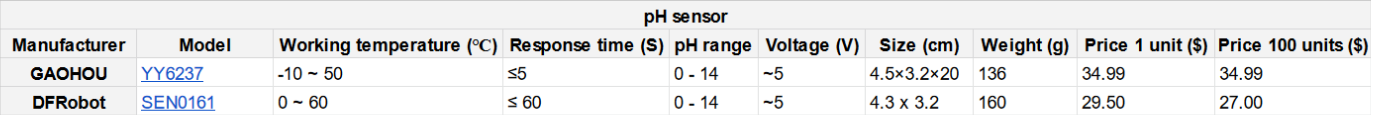
\includegraphics[width=\linewidth]{images/ph-sensor-comparison.png}
    \caption{pH Sensor comparison}
    \label{fig:pH Sensor Comparison}
\end{figure}

\begin{figure}[h]
    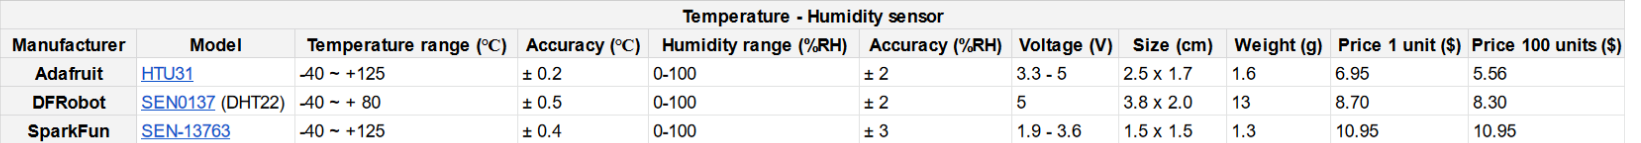
\includegraphics[width=\linewidth]{images/temp-hum-sensor-comparison.png}
    \caption{Temperature - Humidity Sensor comparison}
    \label{fig:Temperature - Humidity Sensor Comparison}
\end{figure}

\begin{figure}[h]
    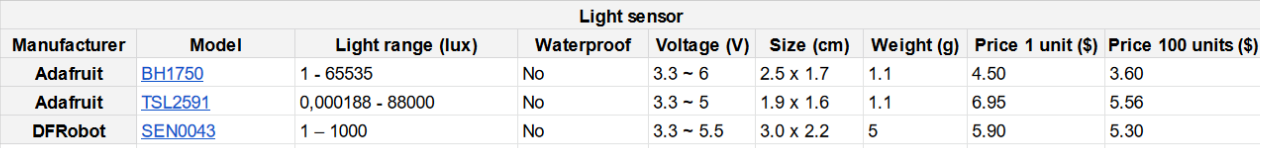
\includegraphics[width=\linewidth]{images/light-sensor-comparison.png}
    \caption{Light Sensor comparison}
    \label{fig:Light Sensor Comparison}
\end{figure}
\subsection{MCU board}
\subsection{Battery}
\subsection{Computing platforms}
\subsubsection{Arduinos and alternative platforms}
\subsubsection{Edge platforms}
\subsubsection{Cloud options}
Azure IoT Hub, AWS, IBM Cloud, Google Cloud \dots
\subsection{Data format}
JSON ? 
\subsection{Device-Edge communication protocols}
Classic Bluetooth, BLE \dots

\subsection{Edge-Cloud communication protocols}
IoT Hub allows devices to use alternative protocols for Edge-Cloud communications, such as HTTP, MQTT and AMQP. In this section we will try to compare each of those protocols and see which ones would suit our project the best.

\subsubsection{MQTT} is a communication protocol with features specifically targeted at IoT solutions. With a small code footprint and low network bandwidth requirements, it is designed as a lightweight publish/subscribe messaging transport that is perfect for linking remote devices.\\
The ease and flexibility with which solutions can be developed is one of MQTT's best features. Multiple clients can produce and share information with back end systems and each other thanks to the publish-subscribe paradigm.

\subsubsection{AMQP} is a messaging protocol which was created to be a non-proprietary method of connecting applications and was not targeted at IoT solutions. It is used on field and cloud gateways to take advantage of connection multiplexing across devices. One of its benefits is that, while being a complicated messaging system, it is lightweight, has little overhead, and uses minimal CPU and RAM. \\
For general purpose message queuing, AMQP offers more flexibility than MQTT, at the expense of some efficiency and complexity.However it places a strong emphasis on message delivery that adds to the overhead eventually.

\subsubsection{HTTP} is a heavy text-based protocol working on a request/response model. A client sends a request to the server, and the server sends back a response.\\
The main benefit of HTTP for use in IoT is its familiarity to developers which are likely to have had implemented web solutions of one kind or another. A consequence of this is the availability of client libraries and servers. Additionally it is scalable and can be used with multiple devices.\\


As MQTT was designed for IoT solutions it fits many more IoT scenarios than its counterparts. \\
Will and retained messages are two MQTT capabilities that AMQP does not directly support. Moreover, mistakes might be made when configuring routing topologies of AMQP, which is impossible in the more straightforward MQTT environment.\\
The cost of connection setup is a small drawback of MQTT versus HTTP. This overhead may be higher than HTTP if each TCP session only sends one message. However, because this is not a typical IoT case, MQTT soon becomes advantageous when several messages are transmitted and received within the same TCP session. HTTP also needs more power and memory to function than MQTT.\\

Considering the advantages and disadvantages of the different protocols listed above and taking into account the comparison table. It seems like the best protocols to implement for the HPCS would be MQTT or HTTP protocols with a preference for MQTT.